\documentclass[11pt,a4paper]{article}

\usepackage[margin=25mm]{geometry}
\usepackage{times}
\usepackage{microtype}
\usepackage{amsmath,amssymb}
\usepackage{graphicx}
\usepackage{booktabs}
\usepackage{caption}
\usepackage[hidelinks]{hyperref}
\usepackage{xcolor}

\graphicspath{{figures/}}

\captionsetup{font=small,labelfont=bf,skip=6pt}

\title{Action history, not a separable prior:\\
a control-heavy decode of the IBL block task in eight regions}
\author{IBL neuromatch analysis pipeline}
\date{23 August 2026}

\begin{document}
\maketitle

\begin{abstract}
Findling, Hubert et al.\ (Nature 2025) report that a Bayes-optimal prior is
decodable from 20--30\% of mouse brain regions in the International Brain
Laboratory (IBL) block task. We asked the same question in eight regions
spanning that hierarchy, matching their target (Bayes-optimal prior),
pre-stimulus window ($-600$ to $-100$\,ms), interleaved cross-validation, and
pseudosession null --- and added the control their paper reports beside the
test rather than inside it. Mice use both the block prior and recent
choice/reward history (held-out accuracy $82.7\%$; history still significant
at lag~5). Raw pre-stimulus counts in caudoputamen (CP), primary and secondary
motor cortex (MOp, MOs) and ventrolateral orbitofrontal cortex (ORBvl) beat
the pseudosession null after FDR. After residualising those counts on
choice/reward history, excess $R^2$ is negative in every region and no session
survives. A decoder that never sees a spike (history alone) yields excess
$R^2 \approx 0.55$--$0.67$. Aligning the window with Findling et al.\ does not
change this pattern. The licensed claim is narrow: in these eight regions,
with a linear decoder in this window, no prior signal separable from action
history was found. It does not license that the Findling result is an
artefact.
\end{abstract}

\section{Question}

Mice in IBL \texttt{ephysChoiceWorld} report the side of a visual grating.
Stimulus side is drawn with $P(\text{left})\in\{0.2,0.8\}$ in blocks of
variable length (mean $\approx 50$ trials). A normative observer can track
$P(\text{next stimulus on the right})$ with a forward filter; that quantity is
the Bayes-optimal prior. Findling et al.\ decode it from Neuropixels activity
in the inter-trial interval and conclude that it is represented at every
processing level, from LGd and VISp through motor cortex to ACAd and ORBvl
\cite{findling2025}.

Block identity and the animal's own recent choices are collinear for almost
the whole session. A decoder can look like a prior decoder while only reading
the last action and its reward. We put that check inside the significance
test.

Two reviewer-facing issues were also closed in this pass: a Python
\texttt{and} bug in fold metadata (\texttt{n\_test\_sessions}), which did not
change any Model~1 number; and the prestimulus window, previously $-400$ to
$0$\,ms, now matched to Findling et al.'s main window of $-600$ to
$-100$\,ms.

\section{Pipeline methodology}

Each stage below states the goal, the algorithm, and what we actually ran.
Conventions (regions, window, QC, protocol filter) live in one file,
\texttt{config.py}. Downstream code imports them; they are not restated per
module.

\subsection{Conventions and data access}

\textit{Goal.} One set of analysis choices, applied identically to every
session, so a window or QC change cannot silently affect only one stage.

\textit{What we did.} Eight Allen CCF regions spanning Findling et al.'s
hierarchy (LGd, VISp, MOs, MOp, ACAd, ORBvl, CP) plus CA1. Sessions must be
block-structured \texttt{ephys}; bandit, opto and passive protocols are
dropped. Units require IBL good-unit QC (\texttt{label}=1). Region membership
uses the CCF descendant set (layers and subnuclei), not string equality.
Pre-stimulus window: $-600$ to $-100$\,ms (extract schema~2). History lags:
$k=1{\ldots}5$. \texttt{one\_client.py} talks to the public Alyx mirror
non-interactively.

\subsection{Survey (\texttt{insertions.py}, \texttt{survey.py})}

\textit{Goal.} Know, before downloading spike trains, which insertions exist,
which protocols are the real block task, and which regions are underpowered
($<3$ subjects or $<5$ sessions).

\textit{Algorithm.} Alyx REST search by atlas acronym. Each insertion gets a
protocol verdict with a reason, so exclusions are counted rather than silent.
Cluster tables (\texttt{clusters.*}, \texttt{channels.*} only) and trial
counts are cached. Coverage, overlap and region-pair matrices are written to
\texttt{data/survey/}.

\textit{What we did.} Ran this over the public 2024 release. Example coverage
among insertions that pass the filter and have good units: CP 107 sessions /
76 subjects; CA1 247 / 164; ORBvl 13 / 11. No spike trains are downloaded
here.

\subsection{Extraction (\texttt{behavior.py}, \texttt{spikes.py},
\texttt{covariates.py}, \texttt{extract.py})}

\textit{Goal.} One on-disk schema per session: trials aligned with
pre-stimulus population counts and history regressors, so a later decoder
cannot mix rows.

\textit{Algorithms.}
\begin{itemize}
\item \textbf{Trials.} Required columns must exist or the session fails.
Choice sign is IBL's: $-1$ = right. Derived columns:
\texttt{signed\_contrast}, \texttt{prior\_bias\_right}$=0.5-p_L$,
reward-gated history $r_{t-k}$ and unrewarded history $u_{t-k}$ at lags
$1{\ldots}5$. Omissions are dropped \emph{before} shifting so they do not
inject NaNs into an otherwise valid lag.
\item \textbf{Spikes.} A cluster inherits its peak channel's CCF id. Counts
in the prestimulus window are \texttt{searchsorted} per cluster relative to
\texttt{stimOn}. Without a QC label the insertion is refused, not filled with
MUA.
\item \textbf{Covariates.} Wheel velocity (resampled at 1\,kHz), whisker
motion energy and pupil diameter, each reduced to a scalar on the \emph{same}
window as the counts.
\end{itemize}

\textit{What we did.} Extracted 84 sessions to \texttt{data/sessions/<eid>/}
with schema~2. Manifests: 78 \texttt{complete}, 6 \texttt{complete\_no\_units}.
Raw spike trains are deleted after counts are written. Decode cuts then keep
pairs with $\ge 3$ good units and $\ge 150$ finite trials (70 sessions, 110
session$\times$region pairs, 49 mice).

\texttt{sanity\_check.py} asserts window-edge inclusion, trial/count
alignment and wheel-velocity sign on synthetic trains and against ONE, so an
off-by-one would not later look like a scientific effect.

\subsection{Stage 1 --- behaviour (\texttt{behavior\_models.py})}

\textit{Goal.} Establish, without spikes, that mice use \emph{both} the block
prior and recent choice/reward history. If history is unused, Stage~2's
confound control is unnecessary. If the prior is unused, there is no
behavioural prior to look for in the brain.

Pilot: 80 sessions, 50 subjects, 12 labs; 53{,}161 trials (45{,}961 biased).

\paragraph{Model 1: history GLM.}
Logistic regression of \texttt{choice\_right} on signed contrast, block
prior, and $(r_{t-k}, u_{t-k})$ for $k=1{\ldots}5$. Nested 5-fold CV is split
at the \emph{session} level so a fold never sees half of a session; the inner
loop only chooses L2 strength $C$. An unregularised cluster-robust fit on the
full set supplies readable coefficients. Held-out accuracy $82.7\%$,
pseudo-$R^2=0.433$. A Python \texttt{and} bug in the stored
\texttt{n\_test\_sessions} was fixed and Model~1 re-run; every number was
unchanged (16 test sessions per fold).

\paragraph{GLM-HMM.}
Three-state Bernoulli GLM-HMM (engaged / left-biased / right-biased). Used
only to label engaged trials for Model~2, not as a neural filter. The engaged
state has near-zero bias and the steepest contrast slope ($38\%$ of trials at
posterior $\ge 0.8$).

\paragraph{Model 2: belief models.}
Four single-trial-update models of how a prior evolves (Bayes-optimal,
fixed-rate, two-rate, surprise-scaled), fit per session by MLE.
Train/test is temporal, not shuffled: shuffling would leak the future through
the belief recursion. Action $a_t\in\{0,1\}$ so $\pi_t$ stays in $(0,1)$.
On engaged trials Bayes-optimal wins; on all trials a fixed-rate kernel wins.
This pass did not re-fit GLM-HMM or Model~2.

\subsection{Stage 2 --- prior decode, four generations}

The headline test is generation 4. Generations 1--3 are why that test is
shaped the way it is.

\paragraph{v1 \texttt{decode.py} (superseded).}
\textit{Goal.} Decode Stage~1's winning belief $\hat\pi$ from pre-stimulus
counts. \textit{Algorithm.} Ridge on GLM-HMM engaged trials only; contiguous
time-block CV; $R^2$ compared to zero. \textit{Outcome.} Negative $R^2$
everywhere. Three confirmed causes: per-session hazard MLE pinned
$\hat\pi$ at $0.5$ in about half of sessions; engaged-only cut $N$ by
$\sim$60\% and left scattered runs; contiguous folds have a ``predict the
training mean'' baseline of $R^2=-0.54$, so zero was the wrong floor.

\paragraph{Controls \texttt{stage2\_controls.py}.}
\textit{Goal.} Tell ``no prior in the data'' from ``the decoder is blind.''
\textit{Algorithm.} Same counts, same ridge, targets whose decodability is
already known. \textit{Outcome.} Trial index $R^2=0.64$ (alignment and
drift); previous choice above chance; ground-truth block above chance in
95\% of pairs; $\hat\pi$ still $\approx 0.02$. Pipeline exonerated; target
and CV scheme indicted. These numbers are a smoke test, not a significance
test (interleaved CV leaks).

\paragraph{Null \texttt{pseudosessions.py} / \texttt{stage2\_null.py} (v2).}
\textit{Goal.} A $p$-value that prices in autocorrelation and session drift.
\textit{Algorithm.} Draw a fresh block sequence from the rig's own process
(90-trial $p_L=0.5$ opener; then $0.2/0.8$ alternating; lengths truncated
exponential on $[20,100]$, mean $\approx 50$), keep the real neural matrix,
score real and 200 fakes on shared interleaved folds. Each target, including
each fake, chooses its own ridge $\alpha$ by GCV so the null is not denied
the tuning the real target got. $p=$ fraction of fakes with $R^2$ at least
as high. \textit{What v2 still decoded.} Raw \texttt{probabilityLeft}, not
the Bayes-optimal prior, and without removing history from the neurons.

\paragraph{Pseudo-population \texttt{pseudopopulation.py} (v3).}
\textit{Goal.} Ask whether a region is underpowered at 10--51 simultaneous
units. \textit{Algorithm.} Pool QC-passing units across sessions (CP 51
$\to$ 770). Each null draw rebuilds the population from a new block sequence;
permuting labels would destroy the drift confound and centre the null at
chance. \textit{Outcome.} A behaviour-only decoder reaches AUC
$0.985$--$1.000$ with no spikes. Pooling amplified the history confound
rather than a prior signal. Noise correlations are destroyed by construction,
so this answers coverage, not mechanism.

\paragraph{Headline \texttt{prior\_decode.py} (v4).}
\textit{Goal.} Match Findling et al.\ on target, window, CV, $R^2$ and
pseudosession null, and put history residualisation \emph{inside} the test.
\textit{Algorithm.} Target $=$ Bayes-optimal prior with fixed hazard
$h=0.02$ (not a per-session MLE). Window $-600$ to $-100$\,ms. Same
pseudosession machinery as v2. Three feature sets, identical target and
null:
\begin{center}
\small
\begin{tabular}{@{}ll@{}}
\toprule
Name & How to read it \\
\midrule
\texttt{counts} & pre-stimulus spike counts (upper bound) \\
\texttt{residuals} & counts after removing choice/reward at lags 1--2
  (the claim) \\
\texttt{confounds} & history alone; no spikes \\
\bottomrule
\end{tabular}
\end{center}
Session $p$-values are combined with Fisher's method and FDR-corrected
across the eight regions. Findling et al.\ regenerate stimuli but not
choices, so real action history stays in the neurons while the fake prior is
unrelated to it; they report that dependence separately. We scored it as a
third decoder.

\textit{What we ran.} 84-session re-extract (schema~2), then
\texttt{prior\_decode} with 200 pseudosessions. Backup of the $-400$ to
$0$\,ms summary kept for Fig.~\ref{fig:window}.

\subsection{Stage 3 --- reversal (\texttt{reversal.py})}

\textit{Goal.} The one place prior and history are opposed: the first trial
after a $0.2\leftrightarrow 0.8$ switch. Train on steady state (lag $\ge 10$),
test after reversal. AUC $>0.5$ tracks the new block; $<0.5$ the old one.

\textit{Algorithm.} Per-session decoder; predictions pooled after
within-session standardisation. Primary test is lag~1 (registered as lags
1--5, then narrowed after the behaviour-only curve --- not after any neural
result --- showed lags $\ge 2$ re-acquire the new block through the stimulus).
Opening $0.5\to$ biased is not a reversal. Time course lags 1--15 with
bootstrap intervals over reversals.

\textit{What we ran.} Behaviour-only AUC $0.10$--$0.16$ at lag~1 (design
check passes). Neural counts in CP and MOp beat the null at lag~1; residuals
do not. \textbf{Not re-run after the window change;} Fig.~\ref{fig:reversal}
is the $-400$ to $0$\,ms extract.

\section{The formulas that actually score}

The working idea is one sentence: the next choice is contrast plus the block
prior plus reward-gated action history. Stage~2 applies that same idea to
spikes. The Bayes filter is only the \emph{target}, not the thing that
explains the neural numbers.

\subsection{Choice (Stage 1)}

Let $a_t=1$ if the mouse turned right, $\sigma(x)=(1+e^{-x})^{-1}$. Then
\begin{equation}
P(a_t=1)
=
\sigma\!\Big(
\beta_0
+ \beta_c\,c_t
+ \beta_\pi\,\pi^{\mathrm{block}}_t
+ \sum_{k=1}^{5}
  \big(\beta_k^{r}\,r_{t-k}+\beta_k^{u}\,u_{t-k}\big)
\Big).
\end{equation}
Signed contrast is \(+\)contrast on a right stimulus and \(-\)contrast on a
left one. The block term is \(\pi^{\mathrm{block}}_t=0.5-p_L\), so a
right-favouring block (\(p_L=0.2\)) is \(+0.3\). History splits rewarded and
unrewarded repeats:
\begin{equation}
s_{t-k}=2a_{t-k}-1\in\{-1,+1\},\qquad
r_{t-k}=s_{t-k}\,\mathbf{1}_{\mathrm{rew}},\qquad
u_{t-k}=s_{t-k}\,\mathbf{1}_{\mathrm{unrew}}.
\end{equation}
Every \(\beta_k^{r}\) and \(\beta_k^{u}\) is positive through lag~5
(Fig.~\ref{fig:model1}). Held-out accuracy is \(82.7\%\). This does
\emph{not} kill the prior: \(\beta_\pi\approx +0.99\). It says the mouse
uses both, which is the confound.

\subsection{The same formula on spikes (Stage 2)}

For each unit, ordinary least squares on that session's own trials:
\begin{equation}
\mathrm{counts}_t
=
B_0
+ B_1 a_{t-1}
+ B_2 R_{t-1}
+ B_3 a_{t-2}
+ B_4 R_{t-2}
+ B_5(a_{t-1}R_{t-1})
+ \varepsilon_t,
\end{equation}
\begin{equation}
\mathrm{residuals}_t
=
\mathrm{counts}_t-\widehat{\mathrm{counts}}_t.
\end{equation}
The ridge then decodes the Bayes-optimal prior from \(\varepsilon\). If a
separable prior lived in the population it would remain in \(\varepsilon\).
It does not: excess \(R^2\) is negative in every region
(Fig.~\ref{fig:decode}, middle). The \texttt{confounds} decoder is the
right-hand side of the same regression with no spikes: excess
\(R^2\approx 0.55\)--\(0.67\). History without a brain outruns every neural
decoder, because in this task the prior and recent actions are nearly the
same variable.

The residualisation is fitted once per session, not inside the CV loop. The
regressors are behavioural history only, never the block label, so the
target cannot leak. The test can only understate leftover prior coding, never
invent it.

\subsection{The decode target (Bayes filter, h = 0.02)}

Two hidden block states, \(p(\mathrm{right})=0.8\) or \(0.2\). Entering trial
\(t\),
\begin{align}
P(\mathrm{high}_t)
&=
(1-h)\,P(\mathrm{high}_{t-1}\mid\mathrm{data})
+
h\,P(\mathrm{low}_{t-1}\mid\mathrm{data}),
\\
\pi_t
&=
0.8\,P(\mathrm{high}_t)
+
0.2\,P(\mathrm{low}_t).
\end{align}
After the stimulus is seen, \(P(\mathrm{high})\) is updated by Bayes' rule.
This \(\pi_t\) is Findling et al.'s target and ours. The formula is correct.
The problem is that \(\pi_t\) is collinear with \((a_{t-1},R_{t-1},\ldots)\),
so decoding it from raw counts does not, by itself, mean the population holds
a prior.

\section{Results}

\subsection{Mice use both prior and history}

Model~1, $N=52{,}391$ trials, pseudo-$R^2=0.433$ (Fig.~\ref{fig:model1}).
Signed contrast ($+4.98$) and the block prior ($+0.99$) both move choice.
Rewarded and unrewarded choice history are significant at every lag through
lag~5. Held-out accuracy is $82.7\%$ (mean log-likelihood per trial $-0.394$;
16 test sessions per fold). Behaviour is not ``prior or history''. It is both.
That is the confound Stage~2 has to beat.

The GLM-HMM engaged state sits near zero bias with the steepest contrast slope
(Fig.~\ref{fig:hmm}A; $38\%$ of trials at posterior $\ge 0.8$). On engaged
trials the Bayes-optimal belief model has the best held-out log-likelihood; on
all trials a fixed-rate kernel wins (Fig.~\ref{fig:hmm}B). That is a
behavioural fact, not a neural one.

\begin{figure}[t]
\centering
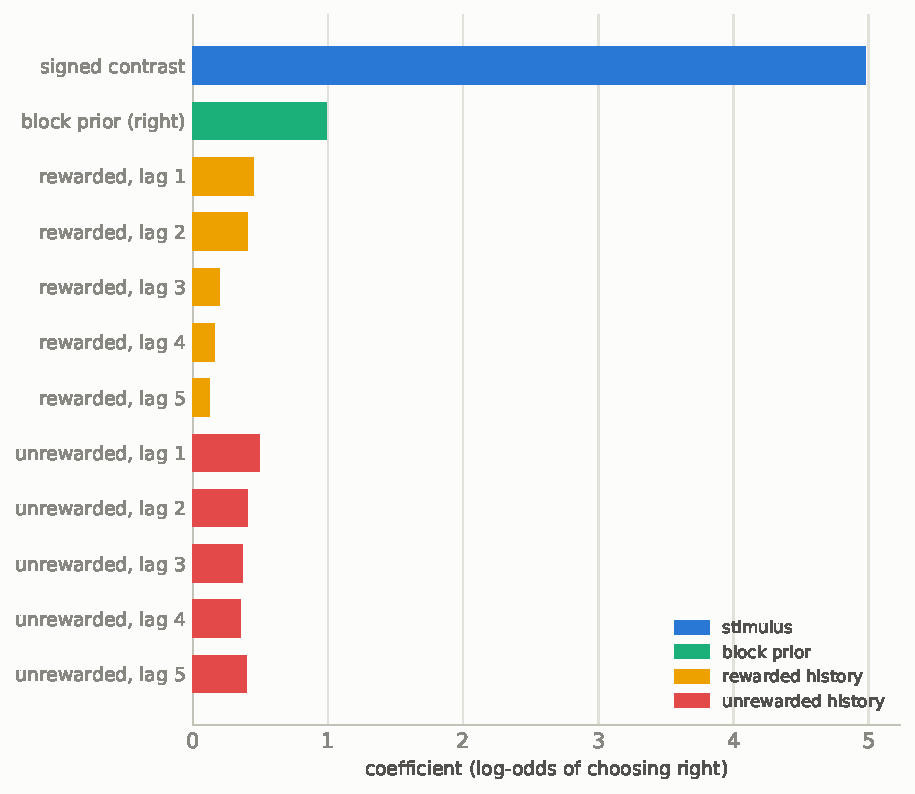
\includegraphics[width=0.72\textwidth]{fig1_model1_coefficients.pdf}
\caption{History GLM of choice (Model~1). Unregularised logistic regression
with session-clustered standard errors. Every history coefficient shown is
$p<10^{-12}$. $N=52{,}391$ trials, 80 sessions, 50 mice.}
\label{fig:model1}
\end{figure}

\begin{figure}[t]
\centering
\begin{minipage}[t]{0.46\textwidth}
\centering
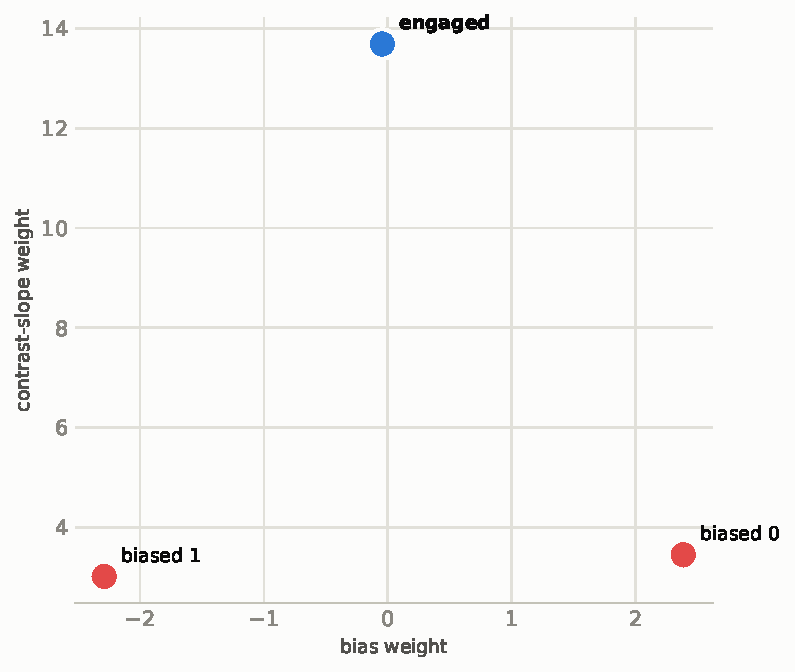
\includegraphics[width=\linewidth]{fig2_glm_hmm_states.pdf}\\[2pt]
{\footnotesize\textbf{A.} GLM-HMM states}
\end{minipage}\hfill
\begin{minipage}[t]{0.50\textwidth}
\centering
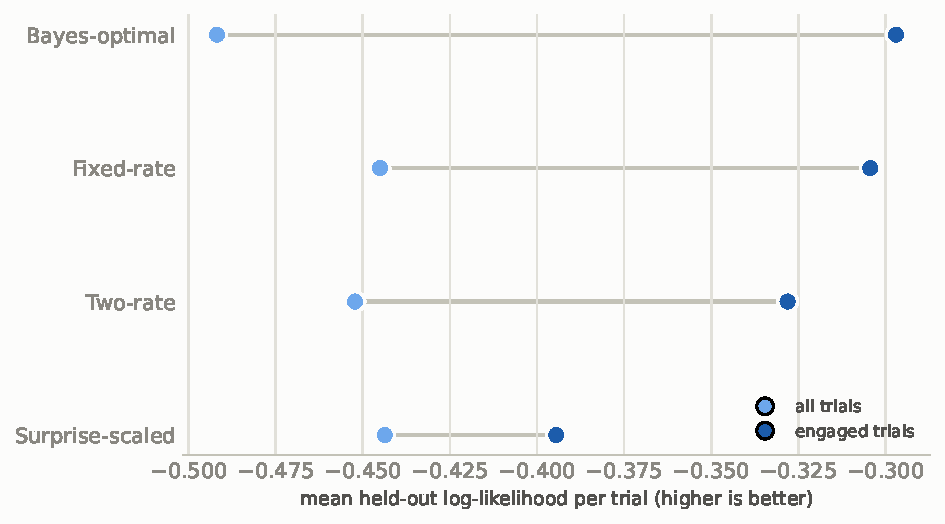
\includegraphics[width=\linewidth]{fig3_belief_models.pdf}\\[2pt]
{\footnotesize\textbf{B.} Belief-model comparison}
\end{minipage}
\caption{\textbf{A.}~Bias versus contrast slope for the three GLM-HMM states.
The engaged state is the one with near-zero bias and the steepest slope.
\textbf{B.}~Mean held-out log-likelihood per trial for four belief models, on
all trials versus engaged-only trials (79--80 sessions).}
\label{fig:hmm}
\end{figure}

\subsection{Counts look like a prior; residuals do not}

Decode set: 110 session$\times$region pairs, 70 sessions, 49 subjects. Window
$-600$ to $-100$\,ms. 200 pseudosessions. Fig.~\ref{fig:decode} is the
headline.

On raw counts, CP, MOp, MOs and ORBvl survive FDR (Table~\ref{tab:decode}).
LGd, VISp, ACAd and CA1 do not. After residualising on choice/reward history,
excess $R^2$ is negative in every region, $n_{\text{sig}}=0$, and BH $q\approx 1$.
History alone (no neurons) yields excess $R^2\approx 0.55$--$0.67$ in every
region, with every session at $p=0.005$ (the floor with 200 nulls). A decoder
that never sees a spike is stronger than any neural decoder in this set.

\begin{figure}[t]
\centering
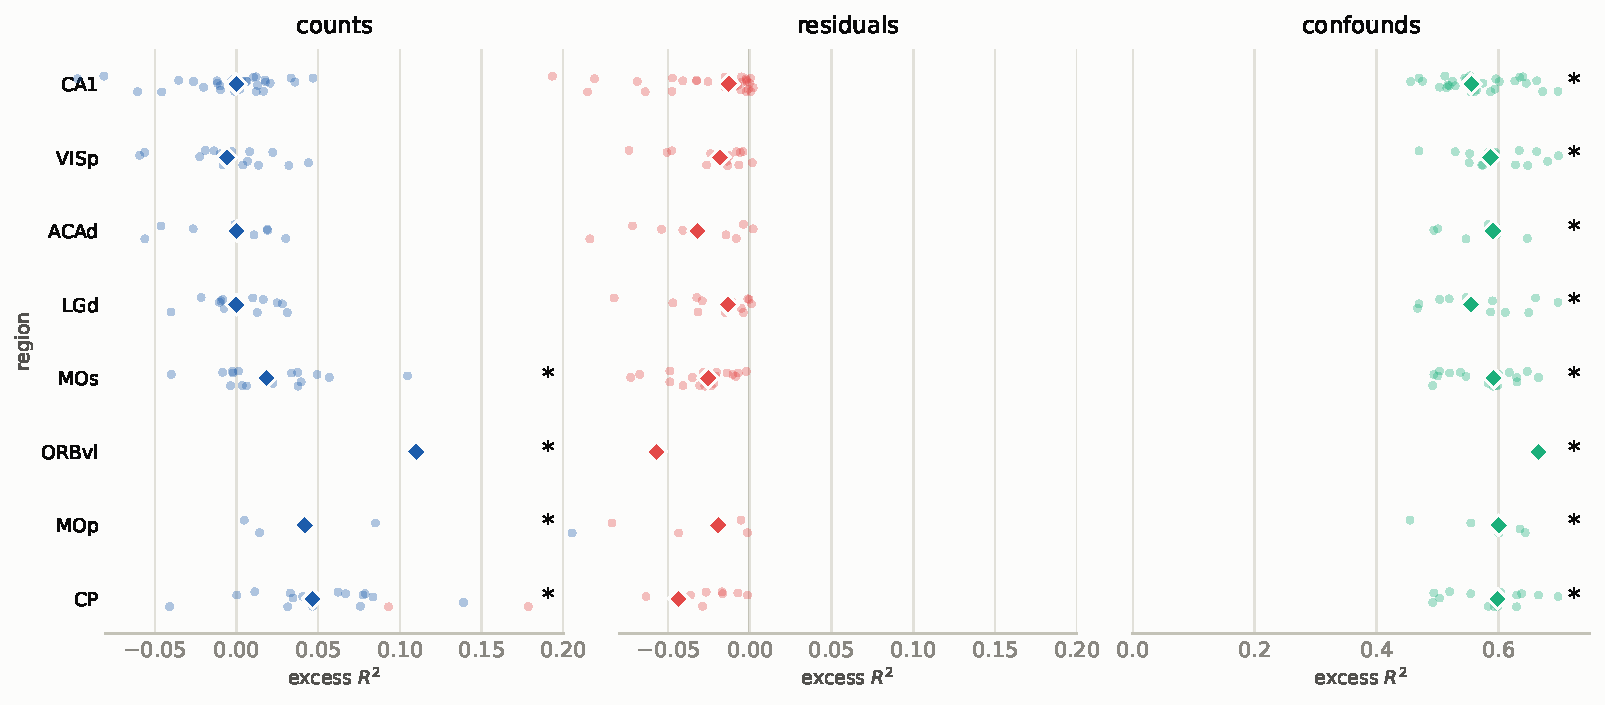
\includegraphics[width=\textwidth]{fig4_decode_excess.pdf}
\caption{Session-level excess $R^2$ for the Bayes-optimal prior
(dots) and regional median (diamonds). Excess $R^2$ is real $R^2$ minus the
median of 200 matched-autocorrelation pseudosessions. Left: raw pre-stimulus
counts. Middle: the same counts after residualising choice/reward history.
Right: history alone, no neural data (note the different $x$ scale). Asterisks
mark regions with Benjamini--Hochberg $q<0.05$. Window $-600$ to $-100$\,ms.}
\label{fig:decode}
\end{figure}

\begin{table}[t]
\centering
\caption{Region-level prior decode, Findling window ($-600$ to $-100$\,ms).
Excess $R^2$ is the median across sessions. BH $q$ is FDR-corrected across
these eight regions.}
\label{tab:decode}
\small
\begin{tabular}{@{}lrrrrrr@{}}
\toprule
Region & $N_{\text{sess}}$ & Excess $R^2$ & BH $q$ & Resid.\ excess & Resid.\ $q$ & Conf.\ excess \\
\midrule
CP    & 15 & $+0.047$ & $6.3\times 10^{-5}$ & $-0.044$ & $1.00$ & $+0.598$ \\
MOp   &  5 & $+0.042$ & $0.012$              & $-0.019$ & $1.00$ & $+0.600$ \\
ORBvl &  1 & $+0.110$ & $0.040$              & $-0.057$ & $1.00$ & $+0.666$ \\
MOs   & 18 & $+0.018$ & $0.040$              & $-0.026$ & $1.00$ & $+0.592$ \\
LGd   & 13 & $0.000$  & $0.84$               & $-0.013$ & $1.00$ & $+0.555$ \\
ACAd  &  9 & $0.000$  & $0.84$               & $-0.032$ & $1.00$ & $+0.591$ \\
VISp  & 17 & $-0.006$ & $0.87$               & $-0.018$ & $1.00$ & $+0.587$ \\
CA1   & 32 & $0.000$  & $0.87$               & $-0.013$ & $1.00$ & $+0.555$ \\
\bottomrule
\end{tabular}
\end{table}

\subsection{Matching the Findling window does not change the story}

Switching from $-400$--$0$\,ms to $-600$--$-100$\,ms slightly raises excess
$R^2$ in CP and MOp, slightly lowers it in MOs, and leaves ORBvl unchanged
(Fig.~\ref{fig:window}). Residuals stay null in both windows. Confound scores
are identical, as they must be (no spikes). The direction is expected if the
counts are mostly an echo of the previous trial's movement and reward: the
Findling window starts earlier and ends $100$\,ms before onset, so it sits
farther from the stimulus edge and closer to the last action.

\begin{figure}[t]
\centering
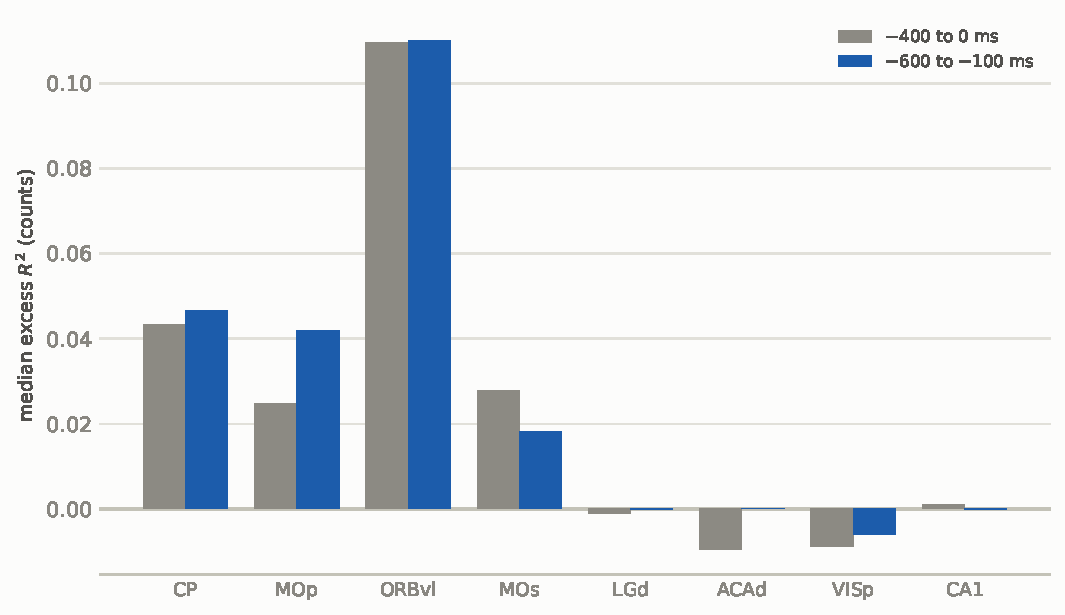
\includegraphics[width=0.82\textwidth]{fig5_window_compare.pdf}
\caption{Median excess $R^2$ of the counts decoder under the project's earlier
window ($-400$ to $0$\,ms) versus Findling et al.'s main window ($-600$ to
$-100$\,ms). Same sessions, same decoder, same null.}
\label{fig:window}
\end{figure}

\subsection{Reversal (old window; not re-run)}

On the first trial after a block switch, a behaviour-only decoder tracks the
\textit{old} block (AUC $\approx 0.10$--$0.16$; Fig.~\ref{fig:reversal}, left).
That is the design check: history and the new prior are opposed, and history
wins. Raw neural counts in CP and MOp beat the null at lag~1 (BH $q=0.035$)
but residual AUC does not ($p=0.26$ and $0.52$). From lag~2 the confound is
already back. These curves use the $-400$ to $0$\,ms extract.

\begin{figure}[t]
\centering
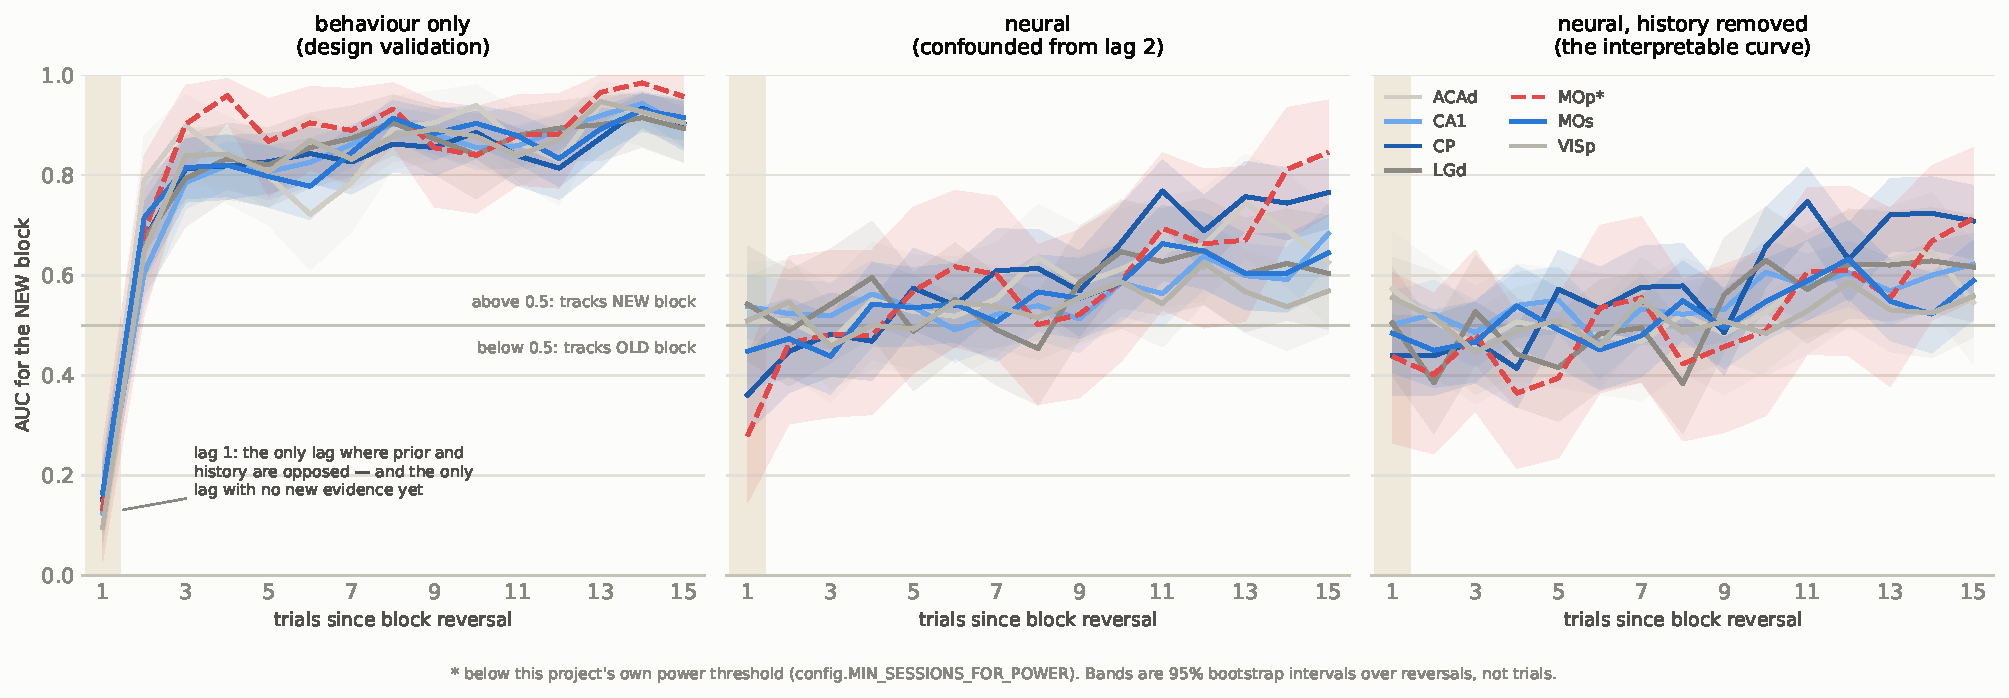
\includegraphics[width=\textwidth]{fig6_reversal_time_course.pdf}
\caption{Decoder AUC for the \emph{new} block as a function of trials since a
$0.2\leftrightarrow 0.8$ reversal. Shaded band: lag~1, the only lag at which
prior and history are opposed. Left: behaviour only. Middle: neural counts.
Right: neural residuals. MOp is underpowered (dashed). \textbf{These panels
were not recomputed after the window change.} Bands are 95\% bootstrap
intervals over reversals.}
\label{fig:reversal}
\end{figure}

\section{How to read this against Findling et al.}

Matched: Bayes-optimal prior (not raw \texttt{probabilityLeft}); window
$-600$ to $-100$\,ms; per-session linear decode; interleaved CV; $R^2$;
pseudosession null; Fisher combination.

Not matched: 8 regions versus 242; 200 pseudosessions versus 1{,}000; no
wheel-stillness screen; no widefield arm; history residualisation inside the
test rather than beside it.

A negative residual result in these eight regions does \emph{not} license
``the Findling result is an artefact.'' It licenses: in these regions, in this
window, with a linear decoder, no prior signal separable from action history
was found. The paper itself reports that past actions influence the decoded
prior for at least five trials and that a correct-versus-error pattern fits an
action kernel better than a Bayes-optimal observer. The disagreement is about
whether that dependence is a side note or the whole signal in the regions we
can power.

ORBvl is one session. ACAd is powered and null on counts. LGd and VISp are
powered and null on counts --- the cleanest contrast with the paper's ``early
sensory too'' claim, and it survives the window alignment.

\section{Code and data}

\begin{itemize}
\item Pipeline: \texttt{ibl\_pipeline/}; window and QC in \texttt{config.py}.
\item Headline test: \texttt{prior\_decode}. Figures: \texttt{make\_figures.py}.
\item Current summary: \texttt{prior\_decode\_summary\_by\_region.csv}.
\item Backup of the $-400$ to $0$\,ms run: the \texttt{\_window400ms} summary CSV.
\end{itemize}

\begin{thebibliography}{1}
\bibitem{findling2025}
C.~Findling, F.~Hubert, International Brain Laboratory, et al.
\newblock Brain-wide representations of prior information in mouse decision-making.
\newblock \emph{Nature} (2025).
\newblock doi:10.1038/s41586-025-09226-1.
\end{thebibliography}

\end{document}
